\documentclass{article}

% if you need to pass options to natbib, use, e.g.:
% \PassOptionsToPackage{numbers, compress}{natbib}
% before loading nips_2018

% ready for submission
%\usepackage{nips_2018}

% to compile a preprint version, e.g., for submission to arXiv, add
% add the [preprint] option:
% \usepackage[preprint]{nips_2018}

% to compile a camera-ready version, add the [final] option, e.g.:
 \usepackage[final]{nips_2018}

% to avoid loading the natbib package, add option nonatbib:
% \usepackage[nonatbib]{nips_2018}

\usepackage[utf8]{inputenc} % allow utf-8 input
\usepackage[T1]{fontenc}    % use 8-bit T1 fonts
\usepackage{hyperref}       % hyperlinks
\usepackage{url}            % simple URL typesetting
\usepackage{booktabs}       % professional-quality tables
\usepackage{amsfonts}       % blackboard math symbols
\usepackage{nicefrac}       % compact symbols for 1/2, etc.
\usepackage{microtype}      % microtypography

\usepackage{graphicx}
\usepackage{hyperref} 
\title{Google Landmark Recognition Challenge, The Ensemble Way }
\usepackage{graphicx}
% The \author macro works with any number of authors. There are two
% commands used to separate the names and addresses of multiple
% authors: \And and \AND.
%
% Using \And between authors leaves it to LaTeX to determine where to
% break the lines. Using \AND forces a line break at that point. So,
% if LaTeX puts 3 of 4 authors names on the first line, and the last
% on the second line, try using \AND instead of \And before the third
% author name.

\author{
  Zahra Jandaghi \\
  Department of Computer Science\\
  University of Georgia\\
  Athens , GA 30605 \\
  \texttt{zahra.jandaghi@uga.edu} \\
  \And
  Omid Setayeshfar \\
  Department of Computer Science\\
  University of Georgia\\
  Athens , GA 30605 \\
  \texttt{omid.s@uga.edu} \\
  \And
  Raunak Dey \\
  Department of Computer Science\\
  University of Georgia\\
  Athens , GA 30605 \\
  \texttt{rd31879@uga.edu} \\
  %% examples of more authors
  %% \And
  %% Coauthor \\
  %% Affiliation \\
  %% Address \\
  %% \texttt{email} \\
  %% \AND
  %% Coauthor \\
  %% Affiliation \\
  %% Address \\
  %% \texttt{email} \\
  %% \And
  %% Coauthor \\
  %% Affiliation \\
  %% Address \\
  %% \texttt{email} \\
  %% \And
  %% Coauthor \\
  %% Affiliation \\
  %% Address \\
  %% \texttt{email} \\
}

\begin{document}
% \nipsfinalcopy is no longer used

\maketitle

\begin{abstract}
 The growing tourism industry demands that tourists be provided with immediate information about the places they visit.
 To address this issue we provide a framework which aims to detect and correctly recognize a landmark from images taken by tourists. 
 We test our model on the google landmark recognition challenge hosted on kaggle. 
 In the google landmark recognition challenge hosted on kaggle. 
 Unlike previous challenges, this task requires classification of 15k classes. We demonstrate the efficacy of our models by training it on the given set of images with ground truth and testing it on unlabelled dataset.
 We obtain xyz score on the kaggle leader board on the testing set.  
 
\end{abstract}

\section{Introduction}

Neural networks have made a lotof progress in recent years owing to the presence of multiple image classification dataset like [1][2].
Many architectures have been designed to specifically address these problems. Networks such as VGG16 [3] and AlexNet [4] have set the premise for more research.
In this project we compare the performance of traditional networks such as the VGG-16  with that of more sophisticated designs such as customized DenseNets adopted from the works of [5] and demonstrate that a customized DenseNet works better.
We further utilize the concept of ensemble learning, by using a multi-pathway Neural network where one of the inputs use clustering information of all the images, and a third branch which is pretrained on the image net dataset. These along with the features extracted form the raw images demonstrate the best performance obtaining a score of xyz on the Kaggle leaderboard.



\subsection{Method}

A neural network based classifier such as the VGG-16 is normally used when it comes to image classification. The standard VGG-16 architecture [figure 1] consists of 
multiple convolution blocks of same filter size followed by a pooling layer to downsample the image by half along both the axis.The first two blocks contain two convolution layers each with filters of size 64 and 128 respectively followed by pooling layers. The third, fourth and fifth branches contain three layers of filters of size 256, 512, and 512. Following this the original VGG paper consists of fully connected layers.
\begin{center}
	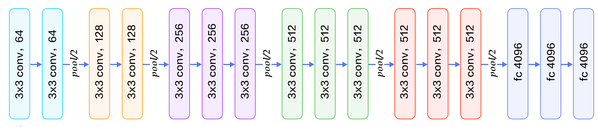
\includegraphics[width=\textwidth]{vgg_16_baseline}
	\captionof{figure 1 :}{Vgg-16 Architecture}
\end{center}
\begin{center}
	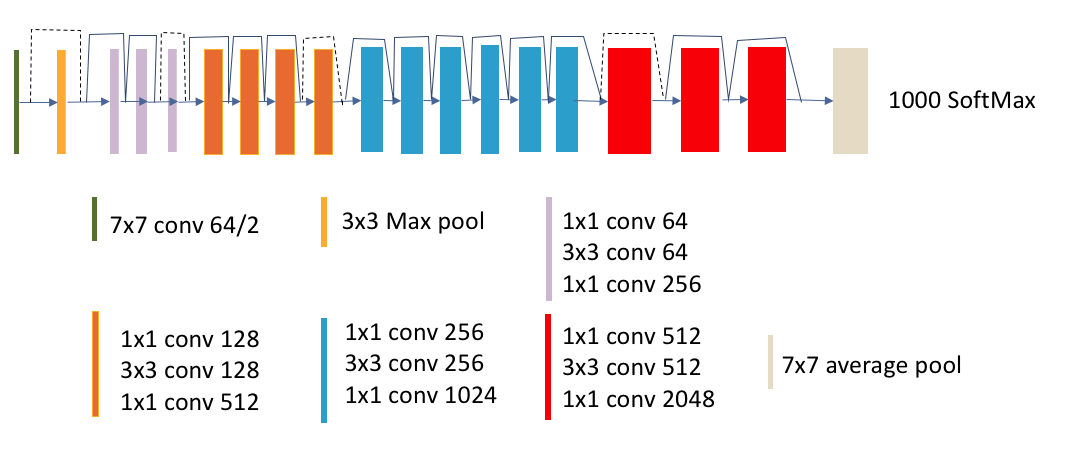
\includegraphics[width=\textwidth]{resnet50}
	\captionof{figure 2 :}{Resnet50 Architecture}
\end{center} 


In order to reduce the number of parameter in the above architecture, we replace the fully connected layers with convolution layers of filter size (1x1). This has two improvement; firstly it reduces the number of parameter drastically since convolution layers share parameters. Secondly the utilization of convolution layers ensure that the spacial relation of the pixels are taken into account during the classification.

We also investigate deeper networks, namely a 36 layer densely connected convolution network. Motivated by the densely connected architecture of [5] where every layer is connected to every other layer in a block, our version of dense network consists of five densely connected block. The first block consists of four convolution layers with 12 feature maps in each block except for the last, which consists of 36 layers. The second till fifth block also consists of 12 convolution filters in each of the seven layers except on the eight layer which increases as 64, 128, 256, 512 for each of the ultimate layer of a dense block. We also introduce batch normalization [6] in order to ensure that the relu activation layers do not blow out of proportion. 

Our intuition suggests that the performance of our classifier can be improved by using hierarchical classification first before fine tuning those features. We anticipate that landmarks which are water based will be different from those which are land based and so on. Thus we cluster our 15000 classes into 100 clusters. This number was chosen arbitrarily and we would like to experiment more on this later. Thus we send to our 36 layer dense-net, the cluster information that image belongs to along with the raw image.

One of the challenges with the task at hand is that many of the images are dominated by faces of the person taking the picture [figure 3] and other objects. This makes the classification task harder since the image contains a lot of noise which we would like to remove. 
\begin{center}
	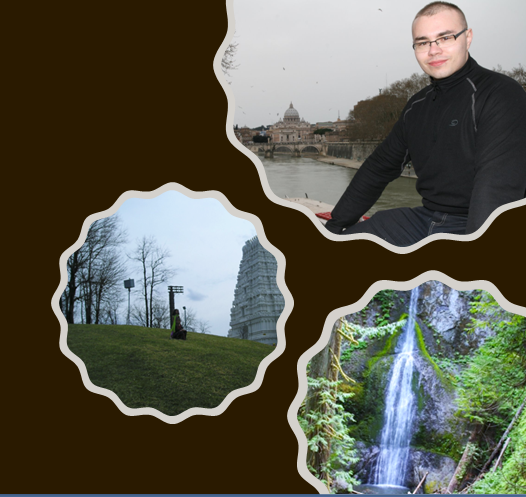
\includegraphics[width=\textwidth]{problems_in_images}
	\captionof{figure 3 :}{Problems with images}
\end{center} 
In order to overcome this issue, we decided to introduce pretrained network to generate a probability map of the contents of the image. We use a pretrained Resnet-50, trained on the Image-Net dataset. The probability map output by this network is used to improve our classification accuracy. The intuition is that some landmarks, local features may dominate which can help identify them. With these two modification we observe that our performance improves by xyz.

Our final network thus has three branches [Figure 4]. The first branch is the same dense net described above. The second branch is a fully connected section of four layers with 32,64,128,256 nodes. The input to this second branch is the cluster number. The third branch is another fully connected section of four layers with 32,64,128,256 nodes. 
The output of the first branch is flattened and merged with the cluster and pretrained network branch and following that we pass the results through a softmax layer with 15000 classes.
\begin{center}
	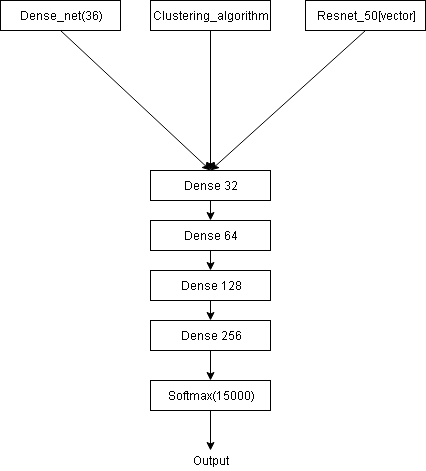
\includegraphics[width=\textwidth]{final}
	\captionof{figure 4 :}{Ensemble Network}
\end{center} 
\subsection{Experiments}

\subsubsection{Dataset}

We evaluate our methods on the images of the Google Landmark recognition challenge hosted on kaggle.[7]
There are 1225029 images in the training set belonging to 15k classes and 117703 testing images whose classes we are to predict. The dataset consists of hashes and URL key mapped to them. The images are of different sizes and resolutions. We use a down loader script from [8]. In total we ended up with x images since some of the links were not active.
We experimented with different image resolution and decided to use 64x64 since the performance didnt vary much for greater resolution. The input to our networks, and the clustering algorithm were images resized to 64x64.



\subsubsection{Experiment Settings}
We used Keras [9] with tensorflow backend [10]to implement our networks. To overcome the overfitting issue we used dropout rate of 0.3 and we also use L2 regularizer to penalize network
weights with large magnitudes and its control hyperparameter  lambda is set to
2e-4. For training, we use the Adam optimizer [11] with a learning rate 1e-3. All
networks run up to 10 epochs.

For our clustering algorithm We have used KMeans algorithm in two settings. In first Setting we clustered 64*64 images into 1000 clusters; later we reduced the number of clusters to 100 as we observed it helps reduce the calculation complexity.

For object classification, we have employed VGG16, VGG19, ResNet50, Inception V3, Xception pretrained models on Imagenet dataset for object classification of our dataset and chosen ResNet50 to continue the experiment with. This desicion was made after running a selected handfull of images through these networks and observing the classificatoin resutls based on number of objects each detected in the images and their coresponding confidence.

\subsubsection{Experiment Results}

We summarize our results in this section. We obtained a rank of 91 on the kaggle leaderboard with a simple dense net described above.
The best performance was obtai
\begin{table}[t]
	\begin{center}
		\begin{tabular}{ |c|c|c|c| } 
			\hline
			Network-type & Training-Accuracy & Kaggle-TestSet\\ 
			\hline
			VGG-16 & 0.0535 & N/A & N/A \\ 
			Dense-Net & 0.5487 & 0.005 &91 \\ 
			Ensemble-Net& 0.4829 & 0.005 & (Rank not updated) \\
			 
			\hline
		\end{tabular}
	\end{center}
\end{table}

\subsubsection{Conclusion }
We explored the Kaggle challenged of Landmark Recognition. It was challenging to handle 15000 classes but we were able to get in the top 50 percentile with our architectures.
Increase in number of features such as clustering and using features of pretrained networks while would be intuitively promising, seemed to make no difference. We suspect this is because it generates too many unrelated features which we can selectively improve.

Click on the following link for the Github-Repo: 
\href{https://github.com/parya-j/team-rope}{Google Landmark Recognition Challenge, The Ensemble Way}
\section*{References}


[1] Krizhevsky, Alex, Ilya Sutskever, and Geoffrey E. Hinton. "Imagenet classification with deep convolutional neural networks." Advances in neural information processing systems. 2012.

[2] Krizhevsky, Alex, and G. Hinton. "Convolutional deep belief networks on cifar-10." Unpublished manuscript 40 (2010): 7.

[3] Han, Song, Huizi Mao, and William J. Dally. "Deep compression: Compressing deep neural networks with pruning, trained quantization and huffman coding." arXiv preprint arXiv:1510.00149 (2015).

[4] Szegedy, Christian, et al. "Rethinking the inception architecture for computer vision." Proceedings of the IEEE Conference on Computer Vision and Pattern Recognition. 2016.

[5] Huang, Gao, et al. "Densely connected convolutional networks." Proceedings of the IEEE conference on computer vision and pattern recognition. Vol. 1. No. 2. 2017.

[6] Ioffe, Sergey, and Christian Szegedy. "Batch normalization: Accelerating deep network training by reducing internal covariate shift." arXiv preprint arXiv:1502.03167 (2015).

[7] https://www.kaggle.com/c/landmark-recognition-challenge

[8] 

[9] chollet2015keras,
title={Keras},
author={Chollet, Fran\c{c}ois and others},
year={2015},
howpublished={\url{https://keras.io}}

[10] Abadi, Martín, et al. "TensorFlow: A System for Large-Scale Machine Learning." OSDI. Vol. 16. 2016.

[11] Zeiler, Matthew D. "ADADELTA: an adaptive learning rate method." arXiv preprint arXiv:1212.5701 (2012).

\end{document}
